\chapter{Parameter Inference}

\section{Motivation}

Building mathematical models of real world phenomenon allows for us to
simulate changes in the world without having to undertake large scale
experiments. However, once we have a model that sufficiently approximates
\emph{P. vivax} transmission
or anything else we are trying to model,
we then need to estimate what the `true' underlying parameters are.
To do this we calibrate the model against real world data such as case counts,
and prevalence surveys. Under frequentist assumptions, there is a `true' set of
parameters that if used in our model, simulated the observed data. Under a Bayesian
assumption, the parameters are considered to be random, and
This chapter explores statistical inference techniques to recover the
parameters, under both the frequentist and Bayesian frameworks.

\section{Frequentist Parameter Estimation}

Assume the model is parametrised by a set of parameters
$\btheta \in \mathbf{\Theta}$ which
we are trying to estimate by considering some observed data
$\mathbf{y}^\obs = (y_1^\obs, \dots, y_n^\obs).$
Consider $\mathbf{f}(\btheta) = (f_1(\btheta), \dots, f_n(\btheta))$
some model simulation of
$\mathbf{y}^\obs.$ Often the observed data has some underlying index set
$x_1, \dots, x_n,$ where $x_i$ might be something like time. In this case
we can also consider the observed data to be
$\{(x_1, y_1^\obs), \dots, (x_n, y_n^\obs)\},$ and the
model simulated data to be
$\{(x_1, f_1(\btheta)), \dots, (x_n, f_n(\btheta))\}.$

\subsection*{Least Squares Estimator}

It is common that models are not random, but instead model the mean behaviour
of a system. In this case, $\mathbf{f}(\btheta)$ is not random. Therefore
we can assume that $y^\obs_i = f_i(\btheta) + \varepsilon_i,$
where $\varepsilon_i$ is a random variable with some (possibly unknown)
distribution, and zero mean.

When the distribution of $\varepsilon_i$ is unknown, a common approach for
estimating $\btheta^{\LS}$ is to take the least squares estimate.

\begin{definition}[Least Squares Estimate]
    The \emph{least squares estimate} $\btheta^{\LS}$ for
    $\btheta$ is
    $$
        \btheta^{\LS}
        := \argmin_{\btheta\in\mathbf{\Theta}}
        \sum_{i = 1}^n (f_i(\btheta)- y_i^\obs)^2.
    $$
\end{definition}

\begin{example}\label{ex:LSE}
    Consider the observed data
    $\{(x_1, y_1^\obs), (x_2, y_2^\obs), (x_3, y_3^\obs)\}
        = \{(1, 2), (2, 4), (3, 4)\},$
    which we assume were generated from the model
    $f_i(\btheta) + \varepsilon_i,$ where
    $f_i(\btheta) = \theta_0 + \theta_1x_i,$ and
    $\E(\varepsilon_i) = 0.$ We derive the least squares estimate of our
    parameters $\btheta = (\theta_0, \theta_1)$ by

    \begin{align*}
        \btheta^{\LS}
        = & \, \argmin_{\btheta}
        [\sum_{i = 1}^3 (f_i(\btheta) - y_i^\obs)^2]           \\
        = & \, \argmin_{\btheta}
        [\sum_{i = 1}^3 (\theta_0 + \theta_1x_i - y_i^\obs)^2] \\
        = & \, \argmin_{\btheta}
        [(\theta_0 + \theta_1 - 2)^2 + (\theta_0 + 2\theta_1 - 4)^2
            + (\theta_0 + 3\theta_1 - 4)^2]
    \end{align*}

    Since the expanded quadratic will have positive coefficients out the front
    of $\theta_0$ and $\theta_1,$ we can solve for $\btheta^{\LS}$
    by

    \begin{align*}
        \mathbf{0}
        = & \, \frac{\partial}{\partial \btheta}
        [
            (\theta^\LS_0 + \theta^\LS_1 - 2)^2
            + (\theta^\LS_0 + 2\theta^\LS_1 - 4)^2
            + (\theta^\LS_0 + 3\theta^\LS_1 - 4)^2
        ]                                        \\
        = & \begin{bmatrix}
                6\theta^\LS_0 + 12\theta^\LS_1 - 20 \\
                12\theta^\LS_0 + 28\theta^\LS_1 - 44
            \end{bmatrix}
    \end{align*}
    And solving these two equations results in $\theta^\LS_0 = 4/3$ and
    $\theta^\LS_1 = 1.$ This can be visually seen in Figure \ref{fig:LSE}
\end{example}


\begin{figure}[htbp]
    \centering
    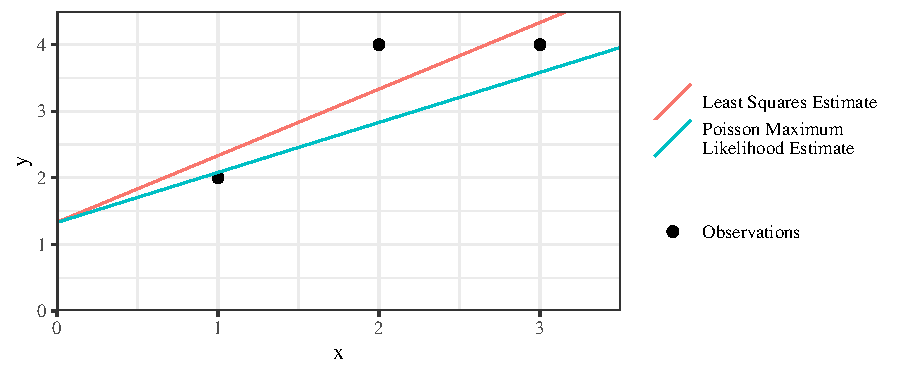
\includegraphics[width=\textwidth]{LS_example.pdf}
    \caption{
        Two linear models of the form
        $f_i(\btheta) = \theta_0 + \theta_1x_i$ fit given the set
        of observations $\{(1, 2), (2, 4), (3, 4)\}$ using the method of
        least squares and maximum likelihood under
        the assumption that the data are independent realisations by a Poisson
        distribution with $\Pois(f_i(\btheta)).$ The least squares estimates
        were $\theta^\LS_0 = 4/3$ and $\theta^\LS_1 = 1.$ The maximum likelihood
        estimates were $\hat{\theta}_0 \approx 1.329$ and
        $\hat{\theta}_1 \approx 0.751.$
    }
    \label{fig:LSE}
\end{figure}

\subsection*{Maximum Likelihood Estimator}

The least square method makes no explicit assumptions about the distribution
of the noise $\varepsilon.$ However if the distribution of $\varepsilon$ is
known (or can be reasonably assumed), we can
explicitly calculate the probability of the data given the parameters.

\begin{definition}[Likelihood function]
    With $\mathbf{y}^\obs$ fixed, the \emph{likelihood function} is
    $$
        \mathcal{L}(\btheta)
        := \Pr(
        \mathbf{f}(\btheta) + \bm{\varepsilon} = \mathbf{y}^\obs
        | \btheta
        ).
    $$
    Particularly, if $f_i(\btheta) + \varepsilon_i$ are independent
    $$
        \mathcal{L}(\btheta)
        = \prod_{i = 1}^n
        \Pr(
        f_i(\btheta) + \varepsilon_i = y_i^\obs
        | \btheta
        ).
    $$
    In the continuous case, if $\mathbf{f}(\btheta) + \bm{\varepsilon}$
    has joint density $p,$
    $$
        \mathcal{L}(\btheta)
        := p(\mathbf{y}^\obs | \btheta).
    $$
\end{definition}

Note that the dependence on $\mathbf{y}^\obs$ is suppressed, but can be
explicitly written as $\mathcal{L}(\btheta|\mathbf{y}^\obs)$
A natural estimate for $\btheta$ is the one that maximises the likelihood
function, as it coincides with the value of $\btheta$ maximises the
probability of the data. Such an estimate is called the maximum likelihood
estimate.

\begin{definition}[Maximum Likelihood Estimate]
    The \emph{maximum likelihood estimate} of $\btheta$ is
    $$
        \hat{\btheta}
        := \argmax_{\btheta\in\mathbf{\Theta}} \mathcal{L}(\btheta)
    $$
\end{definition}

It is often computationally easier to deal with the log-likelihood
$\ell(\btheta) := \ln\mathcal{L}(\btheta).$ Since $\ln$ is a monotonic function,
$\argmax_{\btheta\in\mathbf{\Theta}} \mathcal{L}(\btheta)
    = \argmax_{\btheta\in\mathbf{\Theta}} \ell(\btheta)$

\begin{example}
    Using the same observed data set as Example \ref{ex:LSE}, we assume that
    $y_i^\obs$ were generated independently from
    $f_i(\btheta) + \varepsilon_i \sim \Pois(f_i(\btheta)),$ where
    $f_i(\btheta) = \theta_0 + \theta_1x_i$ as previously defined. Therefore
    the maximimum likelihood estimate of $\btheta$ is
    \begin{align*}
        \hat{\btheta}
        = & \, \argmax \ell(\btheta)                                  \\
        = & \, \argmax_{\btheta\in\mathbf{\Theta}}\sum_{i = 1}^{3}
        y_i^\obs\ln(f_i(\btheta)) -y_i^\obs(\btheta) - \ln(y_i^\obs!) \\
        = & \, \argmax_{\btheta\in\mathbf{\Theta}}\sum_{i = 1}^{3}
        y_i^\obs\ln(\theta_0 + \theta_1x_i)
        - \theta_0 - \theta_1x_i
        - \ln(y_i^\obs!)                                              \\
        = & \, \argmax_{\btheta\in\mathbf{\Theta}}
        2\ln(\theta_0 + \theta_1) - \theta_0 - \theta_1
        + 4\ln(\theta_0 + 2\theta_1) - \theta_0 - 2\theta_1
        + 4\ln(\theta_0 + 3\theta_1) - \theta_0 - 3\theta_1
    \end{align*}
    which we numerically solve to get $\hat{\theta}_0 \approx 1.329$
    and $\hat{\theta_1} \approx 0.751,$ as seen in Figure \ref{fig:LSE}.
\end{example}

\subsection*{Relationship of Least Squares and Maximum Likelihood Estimates}

Although the least squares estimate does not explicitly assume a distribution,
it coincides with the maximum likelihood estimate under the assumption that
the $y_i^\obs$s were has been generated with normal error.

\begin{theorem}
    If $f_i(\btheta) + \epsilon_i \sim N(f_i(\btheta), \sigma^2),$ then
    $$
        \hat{\btheta} = \btheta^\LS
    $$
\end{theorem}

\begin{proof}
    \begin{align*}
        \hat{\btheta}
        = & \, \argmax_{\btheta\in\mathbf{\Theta}}\ell(\btheta) \\
        = & \, \argmax_{\btheta\in\mathbf{\Theta}}
        \sum_{i = 1}^n
        \ln(\frac{1}{\sqrt{2\pi}\sigma})
        -\frac{(f_i(\btheta)- y_i^\obs)^2}{\sigma^2}            \\
        = & \argmax_{\btheta\in\mathbf{\Theta}} \sum_{i = 1}^n
        - \frac{(f_i(\btheta)- y_i^\obs)^2 }{\sigma^2}          \\
        = & \argmax_{\btheta\in\mathbf{\Theta}} \sum_{i = 1}^n
        - (f_i(\btheta)- y_i^\obs)^2                            \\
        = & \argmin_{\btheta\in\mathbf{\Theta}} \sum_{i = 1}^n
        (f_i(\btheta)- y_i^\obs)^2                              \\
        = & \btheta^\LS.
    \end{align*}
\end{proof}

\subsection*{Frequentist Parameter Estimates in Compartmental Models}

Various approaches are possible to parameterise compartmental models.
If the stochastic compartmental model is simple enough, and the number of
people in the model is small enough, then the likelihood
for the stochastic model could be calculated directly. However this is hardly
ever the case, and approximations are usually made.
For a model with a single parameter to fit, the ODE model is
fit to that data point. For example \cite{champagne_using_2022} fit one
unknown model parameter to incidence data.
Alternatively, if there are multiple observations to fit the model to
parameters can be estimated by finding the least squares estimates fit to
the ODE model.
\cite{gani_transmission_2001} fit part of their modified $SEIR$ smallpox model
for using least square estimates.
Another alternative approach
is to assume that the observed data follow a particular distribution
determined by the ODE solution. For example, it is plausible to assume that
daily incidence (case counts) could be distributed according to a Poisson
distribution, with a mean number of cases $\beta \frac{I_t}{N}S_t,$ where $I_t$
and $S_t$ are solutions of the ODEs at time $t$.
Other data such as samples from the population to estimate
prevalence (proportion of those infectious) could be
distributed $\mathrm{Binom}(n, \frac{I_t}{N}).$

\begin{figure}[htbp]
    \centering
    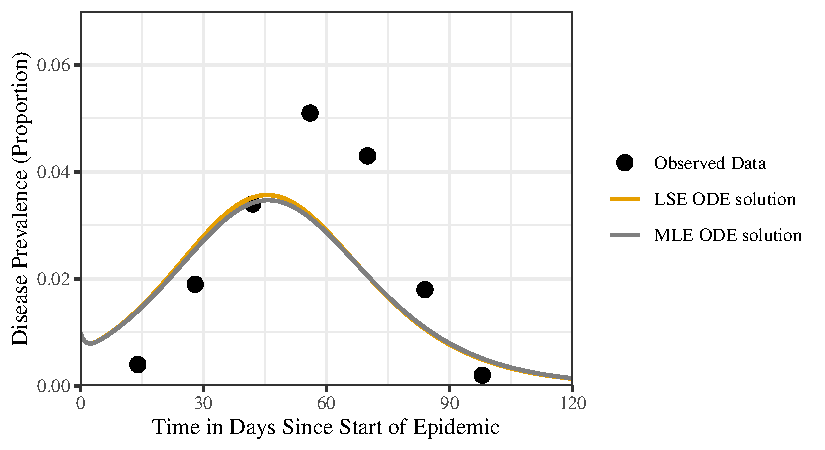
\includegraphics{MLE_SSE_SEIR.pdf}
    \caption{
        An $SEIR$ model fit to some observed prevalence data taken every two
        weeks over a 14 week period, genetated as $I_t/N$ from the $SEIR$
        simulation in Figure \ref{fig:doob_outputs}.
        All parameters were considered known except for $\beta$.
        The least squares estimate (LSE) $\beta^\LS = 0.3516$
        for $\beta$
        was found by solving the model ODEs and numerically minimising the
        square differences between observed prevalences and the ODE prevalences
        (as proportions). Similarly the maximum likelihood estimate
        $\hat{\beta} = 0.3493$ for $\beta$
        was found by assuming the prevalence (times 1000) was binomially
        distributed from 1000 samples with the probability of success being
        equal to $\frac{I_t}{N}.$
    }
    \label{fig:MLE_SSE}
\end{figure}

We demonstrate estimation of one unknown parameter $\beta$ from an $SEIR$ model,
using prevalence data in Figure
\ref{fig:MLE_SSE}. Both $\beta^\LS$ and $\hat{\beta}$ are very close, but do
not fit the data well suggesting fitting the ODEs to a stochastic model
simulation may be a poor choice. This is because at the beginning of an
epidemic the behaviour is very stochastic. Therefore trying to fit an ODE model
to it's stochastic analogue is not necessarily a good idea. The ODEs are more
likely to well approximate the stochastic model when the number of people in
each compartment is high.

\section{Bayesian Parameter Estimation}

In frequentist statistical inference, $\btheta$ is considered to be
fixed, with the observed data $\mathbf{y}^\obs$ assumed to be
generated from a distribution depending on $\btheta.$ Although it is possible
to quantify the uncertainty in parameter estimates through confidence intervals,
frequentist estimates naturally lend themselves to point estimates.
In contrast, inference under a Bayesian
framework assumes that $\btheta$ is also a random variable according to some
pre-known prior distribution. `Evidence' from the observed data then updates
belief about
$\btheta,$ resulting in a posterior distribution of $\btheta,$ described by
Bayes' theorem, namely
$$
    \Pr(\btheta|\mathbf{y}) \propto \Pr(\mathbf{y}^\obs|\btheta)\Pr(\btheta).
$$

Bayesian parameter estimation is still dependent on the likelihood function
$\mathcal{L}$ as expressed in the Bayes' theorem.
With samples from the posterior distribution, we are
able to run our models to capture uncertainty in predicting future scenarios.
For instance, a government may be interested in the number of additional
hospital beds that need to be available to cope with an outbreak of a disease.
If a disease model can be used to approximate outbreaks of the disease,
we can use previous instances of the disease to calibrate our model parameters.
Samples from the posterior parameter distribution, allow
the model to be run multiple times with the varying sets of parameters,
and provide a range of predicted outcomes for the disease. This allows for
confidence in how much investment may be required in the health system.
Similarly, samples from the posterior parameter distribution allow for scenario
modelling such as introducing a new vaccine.

\subsection*{Rejection Sampling}

If we have known ways to sample from the posterior parameter distribution,
then we can use these. However if we have an equation for the probability
distribution, but no way of sampling directly we can sample using rejection
sampling. To sample $X$ through rejection sampling,
we need an explicit way of calculating
$g(x)$ (where $g$ is proportional to the density of $X$), a constant $M$ and
a distribution $p$ such that $Mp(x) \geq g(x)$ with a sampling method
available.

\begin{algorithm}
    \caption{Rejection Sampler}
    \label{alg:rej_samp}
    \begin{algorithmic}[1]
        \State Sample $X^\ast \sim p$
        \State Sample $U \sim \mathrm{Unif}(0, 1)$
        \If{$U \leq \frac{g(X^\ast)}{M p(X^\ast)}$}
        \State \Return $X^\ast$ as a sample from the distribution of $X$
        \Else
        \State Repeat
        \EndIf
    \end{algorithmic}
\end{algorithm}

Under this methodology, the distribution function of $X$ is

\begin{align*}
    \Pr(X = x)
    \propto & \Pr(X^\ast = x , U \leq \frac{g(X^\ast)}{M p(X^\ast)})
    \tag*{where the probabilities may be interpreted as densities}                   \\
    =       & \Pr(U \leq \frac{g(X^\ast)}{M p(X^\ast)} | X^\ast = x) \Pr(X^\ast = x) \\
    =       & \frac{g(x)}{M p(x)} p(x)
    =       & \frac{g(x)}{M}
\end{align*}

as required.

\begin{figure}
    \centering
    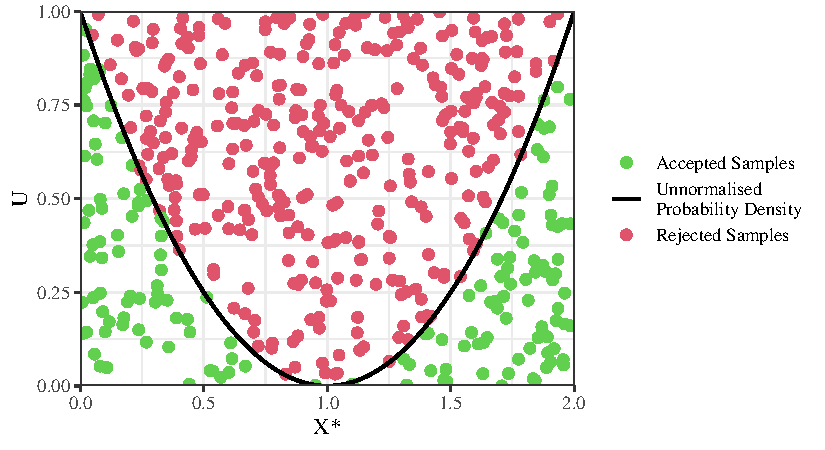
\includegraphics{accept_reject.pdf}
    \caption{
        Samples of $X$ from the unnormalised density $g(x) = (x - 1)^2$ with
        $x\in(0,2)$ using the rejection sampler. $X^\ast\sim\mathrm{Unif}(0,2)$
        and $M = 1.$
        Green dots are samples from
        from $X.$
        Of 500 samples of $X^\ast$, 157 were accepted as samples of $X$.
    }
    \label{fig:accept_reject}
\end{figure}

\begin{example}
    Let $g(x) = (x - 1)^2$ be an unnormalised density function for
    $x \in (0,2).$ $g(x) \leq 1,$ the density of a $\mathrm{Unif}(0,2)$ random
    variable. Therefore to generate samples from $g$ we sample uniformly from
    $X^\ast \sim \mathrm{Unif}(0, 2),$ and then accept the sample if a new
    $U \sim \mathrm{Unif}(0, 1)$ is less than $(X^\ast - 2)^2.$ This is
    demonstrated in \ref{fig:accept_reject}
\end{example}

\subsection*{Monte-Carlo Markov Chain Methods}

Often it is not possible to sample directly from the posterior distribution
$\Pr(\btheta|\mathbf{y})$ using a rejection sampler, as there is no
explicit form proportional to the true density.
Therefore a common way of sampling from the posterior distribution is
to construct a Markov chain that has the same stationary distribution as the
posterior parameter distribution, and take samples from the chain as samples
from the posterior.

\begin{definition}[(Discrete Time) Markov Chain]
    A sequence of random variables
    $X_0, X_1, \dots$
    is a (discrete time) \emph{Markov chain} $\{X_k\}_{k\in\mathbb{N}}$ if for
    all
    $k\in\mathbb{N}$,
    $$
        \Pr(X_{k+1}\in A|X_0, X_1, \dots, X_k) = \Pr(X_{k+1}\in A|X_0, \dots, X_k)
    $$
\end{definition}

We will restrict our focus to time homogeneous Markov chains, that is, where
$\{X_k, X_{k+1}, \dots, X_{k + n}\}$ has the same distribution as
$\{X_{k^\prime}, X_{k^\prime+1}, \dots, X_{k^\prime + n}\}$ for all
$k, k^\prime, n \in \mathbb{N},$ given $X_k = x = X_{k^\prime}$. In other words,
as long as one knows the value at some point in the chain, how far along the
chain someone is has no impact on the distribution along the chain.

\subsection*{Metropolis Hastings}

\begin{figure}[htbp]
    \centering
    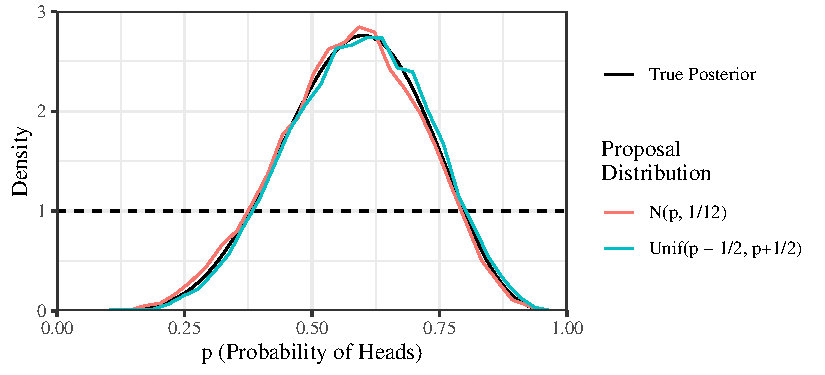
\includegraphics{coin_MH_R.pdf}
    \caption{30,000 samples from the posterior distribution of $p$ using the Metropolis Hastings algorithm. It was assumed that $p\sim \mathrm{U}(0,1)$ and $H \sim \mathrm{Binom}(10, p),$ given $H = 6.$ A uniform and normal proposal distributions were compared.}
    \label{fig:coin_R}
\end{figure}

\begin{figure}[htbp]
    \centering
    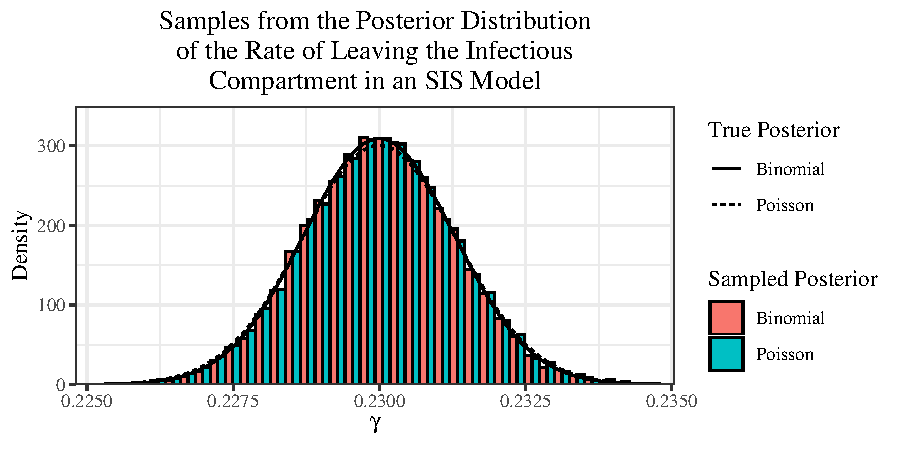
\includegraphics{SIS_gamma_pred.pdf}
    \caption{
        I created this ages ago but I think it's estimating
        $\gamma$ from an SIS model so I'll figure it out and I think it is 
        using metropolis hastings
    }
    \label{fig:SIS_MH_R}
\end{figure}

\subsection*{Gibbs Sampling}

\begin{figure}[htbp]
    \centering
    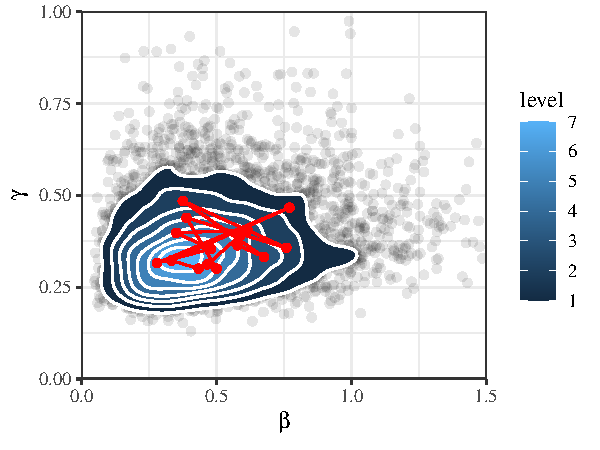
\includegraphics{SIS_gibbs.pdf}
    \caption{Using Gibbs on beta and gamma given an `$R_0$' observation}
    \label{fig:gibbs_R}
\end{figure}

\subsection*{ABC}